% Add "answers" option to print the answers
\documentclass[addpoints, answers]{exam}

\usepackage[utf8]{inputenc}
\usepackage{calc}
\usepackage[dvipsnames]{xcolor}
\usepackage{ifthen}
\usepackage{tcolorbox}

% \makebox[\textwidth]{Name:\enspace\hrulefill}
%  
% \vspace{5mm}
%\makebox[\textwidth]{Instructor’s name:\enspace\hrulefill}

\definecolor{MyLightGray}{gray}{0.60}

\newcommand{\truefalse}
{		\begin{checkboxes}
			 \choice True
			 \choice False. Explanation: 
		\end{checkboxes}
		\vspace{10pt}
}


% Check if 'answers' is an option
\newcommand{\ifanswers}[2]{%
  \ifthenelse{\boolean{exam@answers}}{#1}{#2}%
}



\newcommand{\answerspace}[1]
{
	\ifprintanswers
	\else
		\setlength{\mylength}{10pt}%
		% \vspace{#1\mylength}
		% Make the grey box
		\par\nobreak\noindent
		\makebox[\linewidth][l]{%
			% set inner padding to zero, so only the frame shows
			{\setlength{\fboxsep}{0pt}%
			% draw a color frame, white (or transparent) inside
			\fcolorbox{MyLightGray}{white}{%
			% the inner box has zero width content but fixed height
			\parbox[t][#1\mylength][c]{%
				% subtract twice the frame‐thickness from the full width
				\dimexpr\linewidth-2\fboxrule\relax
			}{\strut}%
			}%
			}%
		}%
		\par
		\vspace{3\mylength}

  	\fi
}
\newlength{\mylength}

\newcommand{\code}[1]{{\texttt{#1}}}

\newcommand{\answer}[1]{\begin{solution}{#1}\end{solution}}




%\usepackage{listings}
\usepackage{color}
\usepackage{lastpage}
\usepackage{verbatim}
\usepackage{fancyvrb}
\usepackage{graphicx}
\usepackage{float}
\usepackage{minted}
\usepackage{multicol}

\newcommand{\includecode}[2][c]{\lstinputlisting[caption=, escapechar=, language=#1]{#2}<!---->}
\RecustomVerbatimCommand{\VerbatimInput}{VerbatimInput}{}

\renewcommand{\solutiontitle}{\noindent\textbf{Solution sketch: }}

\definecolor{SolutionColor}{rgb}{0.8,0.9,1}

\cfoot{Page \thepage\ of \pageref{LastPage}}

\rhead{Initials: \rule{20mm}{0.4pt}}



%%%%%%%%%%%%%%%%%%%%%%%%%%%%%%%%%%%%%%%%
\begin{document}
\fvset{numbers=left,numbersep=3pt}
\thispagestyle{empty}

\begin{center}
	{\LARGE CS 408 Spring 2026 -- Practice Midterm \\}

	\vspace{20mm}
\fbox{\fbox{\parbox{5.5in}{\centering
	\begin{itemize}
          % \item Write your \textbf{name} in the first page and your \textbf{initials in every other page}.
        \item The exam is closed notes, closed book.

        \item The exam should be completed individually: any
          communication with your fellow students is strictly
          prohibited.

	\item Please print or write legibly.

        \item If you have a question, raise your hand and the
          course staff will come to you.

        \item Provide complete and clear but concise
          answers. Any explanations should be thorough.

        \item Answer the questions in the spaces provided. Your answer
          does not need to take up all the space provided; if you run
          out of room, use the empty pages at the back of the exam to
          complete your answer.

        \item Coding questions should be answered in Java, unless
          requested otherwise.

        \item Unless otherwise noted, CFG nodes represent basic blocks.
          % or low-level pseudo-code.
          % \item Unless otherwise noted, assume that questions refer to C code, AT\&T assembly syntax and the x86 architecture.

        \item Please double check that your copy of the exam
          is complete; you should have \pageref{LastPage}
          pages.

        \item You have 75 minutes to complete the exam.
        \end{itemize}
	}}}
\end{center}

\vspace{13mm}
\begin{center}
	\makebox[0.6\textwidth]{
		\combinedgradetable[h][questions]
	}
\end{center}
%\begin{center}\combinedgradetable[h][questions]\end{center}
\vspace{28mm}


\makebox[\textwidth]{\textbf{Name (please print)}: \rule{100mm}{0.8pt} }
%\end{center}

\vspace{10mm}
%\begin{center}
\makebox[\textwidth]{\textbf{PUID}: \rule{40mm}{0.8pt} \hspace{35mm}}
%\end{center}


\begin{questions}

	\newpage
%	\question State whether the following statements are true of false. \textbf{Explain the false statements.}
%	\begin{parts}
%		\part[2]
%		\truefalse
%		\answer{True.}
%
%	\end{parts}




\question Consider the concept of faults, errors and failures.

\begin{parts}

\part[3] What is the difference between an error state and a failure?
  Explain. %
  \answerspace{9} %
  \begin{solution} %
    An error state is an \textit{incorrect internal state of the
      program}, e.g., when an internal variable holds a value it would
    never hold if the program did not conatin a fault.

    A failure is an observable behavior that is inconsistent
    with respect to the expected behavior: the program crashes
    when it should not, or it produces the wrong output).  %
  \end{solution}

\part[3] What is the relationship between an error state and a
  failure? Explain. %
  \answerspace{10} %
  \begin{solution} %
    A program \textbf{must} encounter an error state in order for a
    failure to happenx, i.e., an error state is a \textit{necessary
      precondition} for a failure.

    Importantly, however, not all error states lead to failures.  %
  \end{solution}

\end{parts}

\question Consider the following three approaches to testing a function:
  \begin{itemize}
  \item \textbf{Approach 1:} Run the target program on $N$
    randomly chosen inputs
  \item \textbf{Approach 2:} Run the target program on a
    representative set of $N$ inputs
  \item \textbf{Approach 3:} Run the target program on all inputs
  \end{itemize}

  You can assume N is in the order of tens of thousands.

\begin{parts}

\part[3] Explain the pros and cons of the first ($N$ random
  inputs) and last (all inputs) approaches.%
  \answerspace{11}%
  \begin{solution}%

    \begin{itemize}
    \item Approach 1:
      \begin{itemize}
      \item \textbf{Pros:} Simple and efficient; there is a
        non-zero probability of finding failures if they exist.

      \item \textbf{Cons:} The likelihood of finding errors is
        proportional to the size of the input space and
        becomes vanishingly small as the total number of
        possible inputs grows. A purely random selection
        strategy is likely to miss corner cases.
      \end{itemize}

    \item Approach 3:
      \begin{itemize}
      \item \textbf{Pros:} Comprehensive; will eventually find
        every fault that exists (assuming the function
        terminates on all inputs).

      \item \textbf{Cons:} Testing is unlikely to finish within
        the heat death of the universe.
      \end{itemize}
    \end{itemize}
  \end{solution}

%  \newpage
      \part[3] Describe how a tester might use input space
        partitioning to identify a ``representative set of inputs''
        used by the second approach. %
        \answerspace{9}%
        \begin{solution}%

          A tester partitions the set of inputs into equivalence
          classes and selects a representative input from each class.

          Inputs in the same class are expected to behave similarly,
          while inputs in different classes are expected to behave
          differently.

        \end{solution}

      \part[3] What is the main advantage of the last approach over
        the other two? %
        \answerspace{9} %
        \begin{solution}%
          The main advantage of the third approach is that it is
          \emph{complete}-- since this approach is exhaustive, if a
          failure exists, this approach will find it. Conversely, if
          exhaustive testing does not discover a failure, the function
          is guaranteed to behave correctly.

          In contrast, the other testing approaches are sampling
          techniques, and can only guarantee the absence and/or
          presence of failures on the inputs they have examined. %
        \end{solution}

\end{parts}


% \question Consider the RIP model, as discussed in class.

% \begin{parts}

% 	\part[5] What are the components of the RIP model? What is the relevance of the RIP model and each of its components for testing? Explain.
% 	\answerspace{12}
% 	\begin{solution}
% 		RIP model defines three conditions that must be satisfied for a failure to be observed during testing, specifically:
% 		\begin{itemize}
% 			\item \textbf{Reachability:} The location or locations in the program that contain the fault must be reached.
% 			\item \textbf{Infection:} After executing the location, the state of the program must be incorrect.
% 			\item \textbf{Propagation:} The infected state must propagate to cause some output of the program to be incorrect.
% 		\end{itemize}
% 	}


% 	\part[3] What part is not covered by the RIP model that is c_also important for testing?
% 	\answerspace{12}
% 	\begin{solution}
% 		Revealability. The tester must observe part of the incorrect output.
% 	}


% \end{parts}

\newpage

\question Consider the following function:
  \begin{minted}{Java}
public static int binarySearch(int[] arr, int x) {
  int l = 0;
  int r = arr.length - 1;
  while (l <= r) {
    int mid = l + (r - l) / 2;
    if (arr[mid] == x) {
      return mid;
    }
    if (arr[mid] < x) {
      l = mid + 1;
    } else {
      r = mid - 1;
    }
  }
    return -1; // element not found
}
\end{minted}

\begin{parts}

\part[4] Draw the CFG of this program. Label each node with the basic
  block it represents. Use a range of line numbers when necessary,
  e.g., use L2-7 as the label for a basic block starting at line 2
  and ending at line 7. If a line corresponds to more than one node,
  add a sequential letter suffix starting on ’a’ to distinguish
  them. For instance, if line 7 corresponds to two nodes CFG, you
  \textbf{must} name the first 7a and the second 7b. %

  \answerspace{22} %
  \begin{solution} %
    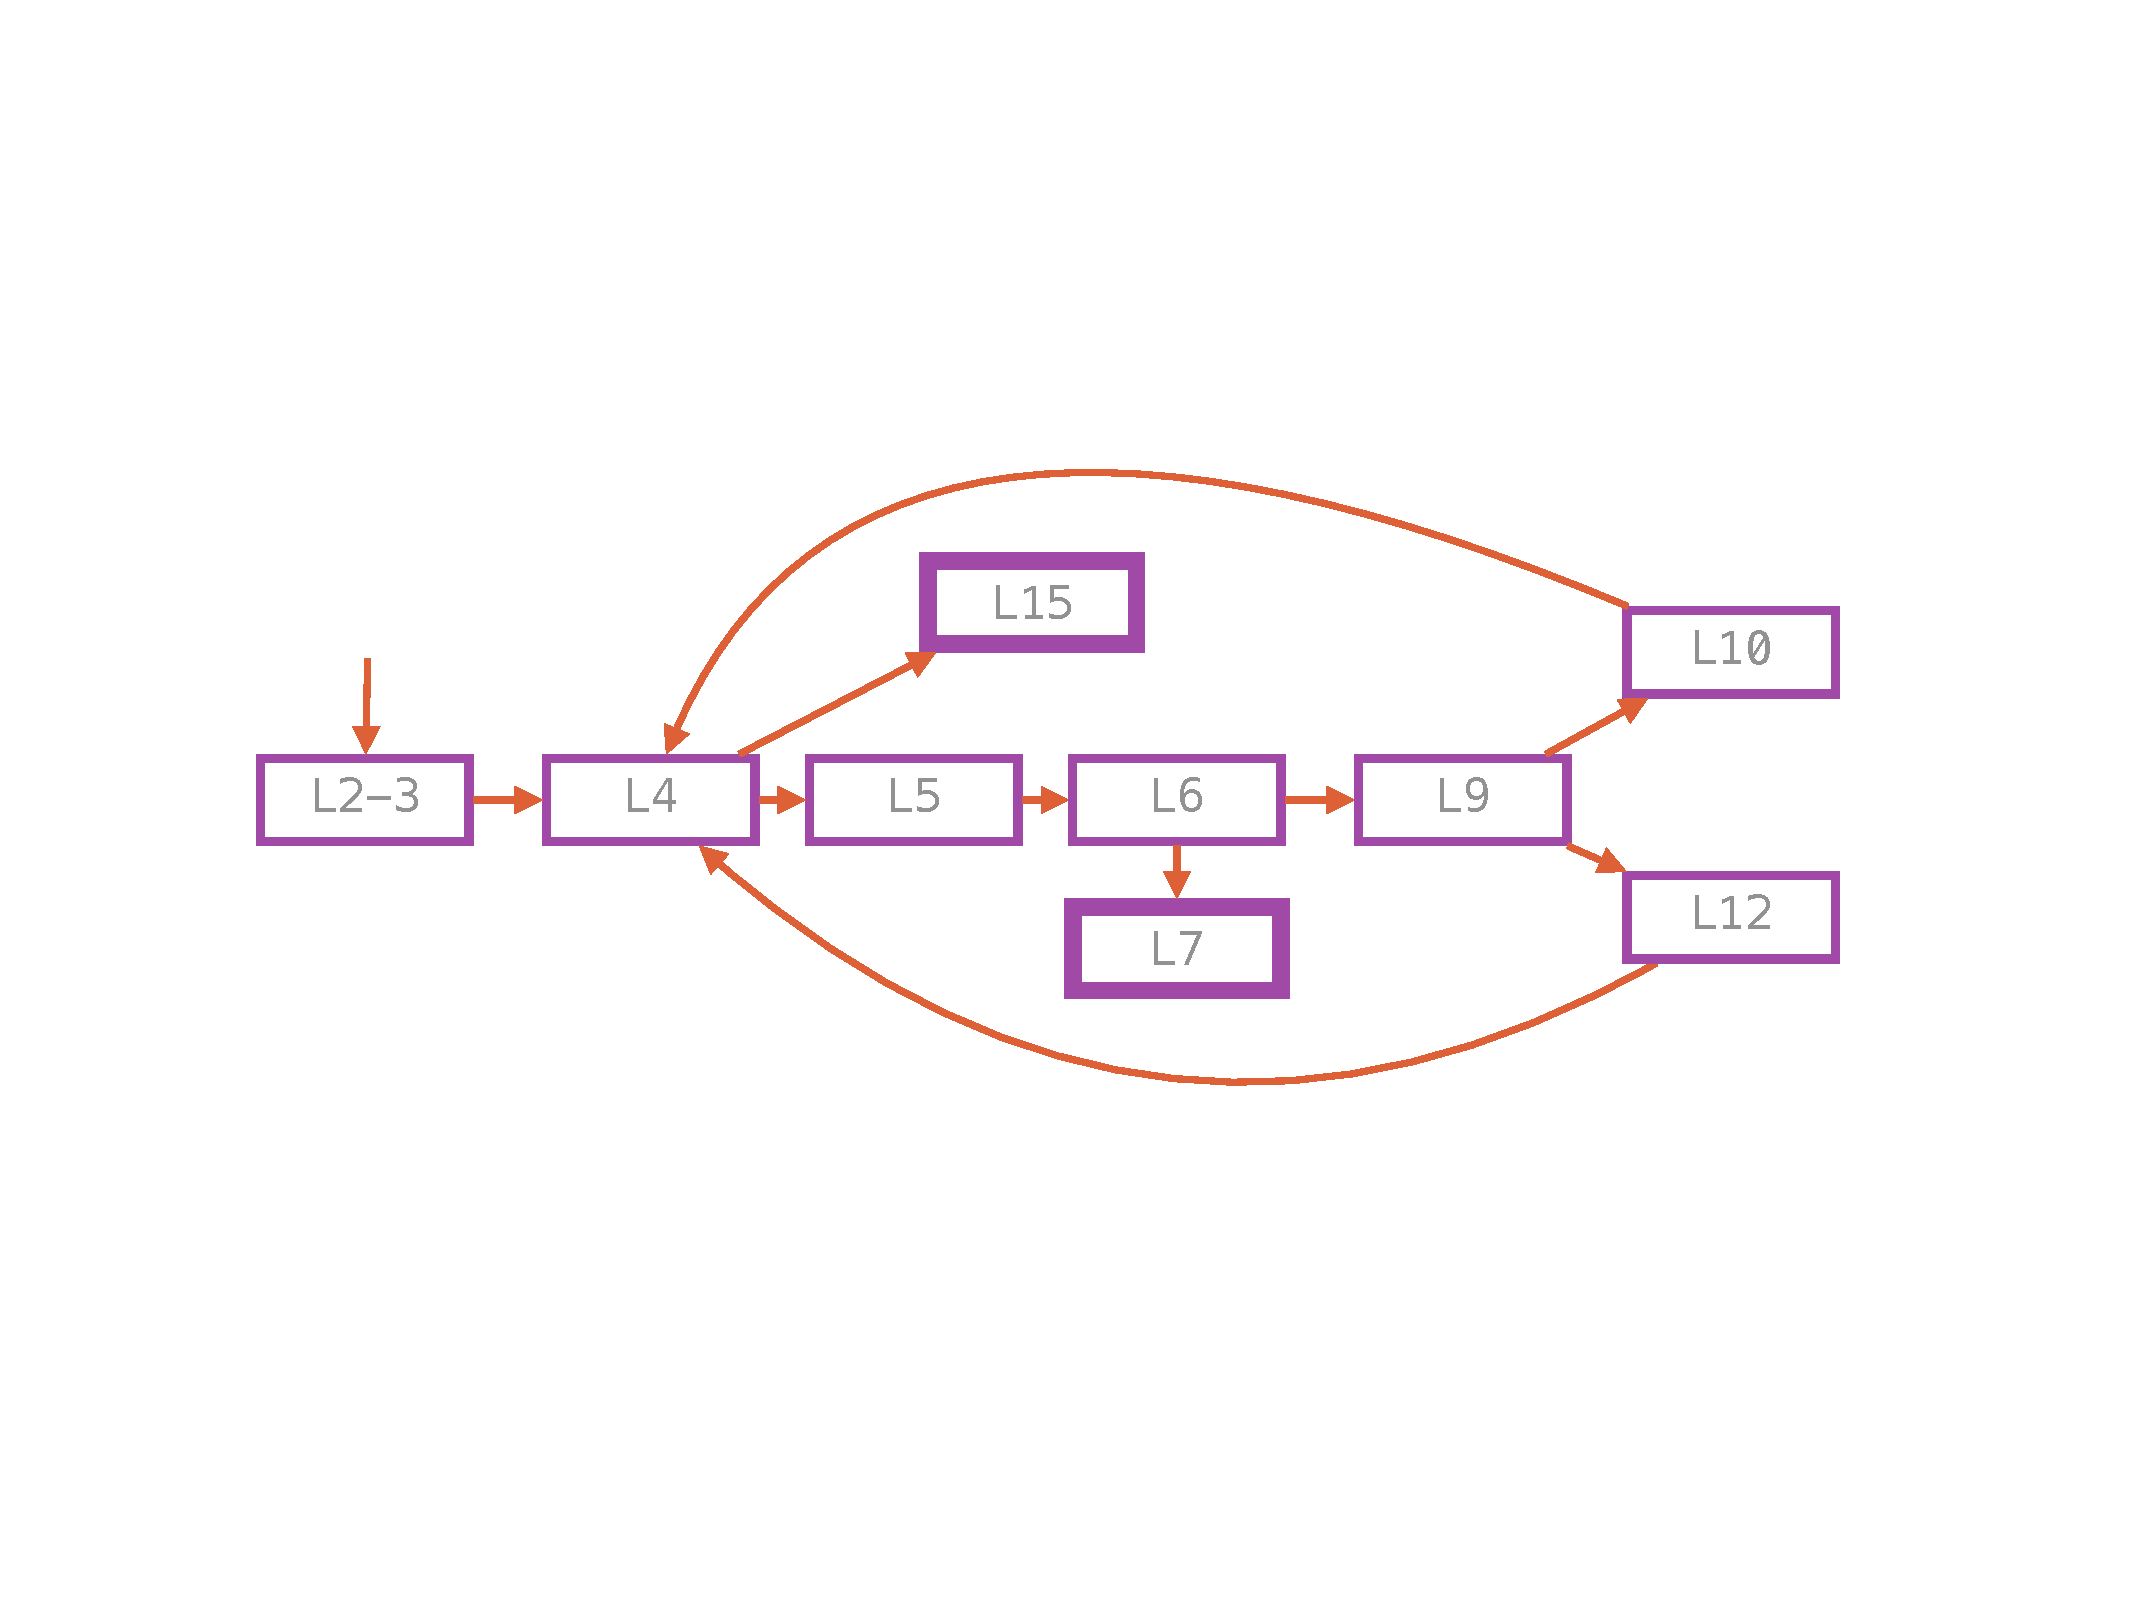
\includegraphics[width=7cm]{figures/sample-midterm-binary-search-cfg.pdf}
  \end{solution}

\part[3] What is a basic block? %
  \answerspace{9} %
  \begin{solution} %
    A basic block is a sequence of consecutive statements that has one
    entry point and one exit point, with no jump to/from the middle.
  \end{solution}

\part[2] Is there any advantage to using basic blocks as opposed to
  statements in CFGs? %
  \answerspace{9} %
  \begin{solution} %
    Yes. It creates a much more compact graph, which is more efficient
    for program analyses. %
  \end{solution}

\part[2] Is there any disadvantage to using basic blocks as opposed to
  single statements in CFGs? %
  \answerspace{9} %
  \begin{solution} %
    For structural coverage analysis there is generally no
    disadvantage. (Other answers are also valid if well justified.)
    % Yes. It is impossible to analyze the program state between statements that are grouped into the same basic block.
  \end{solution}

\end{parts}

\newpage

\question Consider the following Java function:
  \begin{minted}{Java}
public static int indexEven(int[] x, int n) {
 // if x is null, return -1
 // otherwise return the index of the n-th even number in array x
 // so that n=1 returns the first even element, n=2 returns the second
 // *or* return -1 if there is no n-th even number in array x
  if (x == null) {
    return -1;
  }
  int count = 0;
  for (int i = 0; i < x.length; i++) {
    if (x[i] % 2 == 0) {
      if (count == n) {
        return i;
      } else {
        count++;
      }
    }
  }
  return -1;
}
\end{minted}

\begin{parts}
\part[3] State the location(s) of the program fault and explain how
  you would fix the program. Consider only the smallest and simplest
  fix. %
  \answerspace{10} %
  \begin{solution} %
    The simplest explanation\footnote{Other answers are also valid if
      well justified.} is that the fault is on line 6-- by starting
    the \mintinline{Java}{count} at 0, this function will returns the
    $n+1$-th element of the list, since the comment at the start of
    the function indicates that the first even element of the list is
    the $1-th$ one.
  \end{solution}

\part[3] If possible, provide an example of a test input that
  does not cause the fault to execute.  If this is not possible
  explain why.

  \answerspace{10} %
  \begin{solution} %
    If the test input is (\mintinline{Java}{x}$\mapsto$
    \mintinline{Java}{null}, \mintinline{Java}{n}$\mapsto$
    \mintinline{Java}{1}), \mintinline{Java}{indexEven} will return
    on line 6 without executing the fault.%
  \end{solution}

%\newpage

\part[3] If possible, provide an example of a test input that causes
  the fault to execute but no error state to occur. If this is not
  possible explain why. %
  \answerspace{10} %
  \begin{solution} %
    This is not possible for the scenario described above -- the
    initial value of \mintinline{Java}{count} in the correct
    implementation of \mintinline{Java}{indexEven} is always
    \mintinline{Java}{1}!%
  \end{solution}

\part[3] If possible, provide an example of a test input that causes
  the fault to execute, the error to occur, but no failure to
  occur. If this is not possible explain why. %
  \answerspace{10} %
  \begin{solution} %
    If the test input is (\mintinline{Java}{x}$\mapsto$
    \mintinline{Java}{[1, 3, 5]}, \mintinline{Java}{n}$\mapsto$
    \mintinline{Java}{1}), the fault is executed and the initial value
    of \mintinline{Java}{count} is erroneously set to
    \mintinline{Java}{0}, but \mintinline{Java}{indexEven} returns
    \mintinline{Java}{-1}, as expected.%
  \end{solution}

\part[3] If possible, provide an example of a test input that causes
  the fault to execute, the failure to occur, but no error to
  occur. If this is not possible explain why. %

  \answerspace{10} %
  \begin{solution} %
    This is impossible: as described in the answer to question 1b
    above, an error state \emph{must} be encountered in order for a
    failure to be observed. %
  \end{solution}

  %\newpage

\part[4] Describe and explain the condition that an input must satisfy
  for the error state to occur. %
  \answerspace{10} %
  \begin{solution} %
    This error state happens whenever \mintinline{Java}{x} is
    non-null.
  \end{solution}

\part[4] Describe and explain the condition that an input must
  satisfy for the failure to occur. %
  \answerspace{10} %
  \begin{solution} %
    A failure will always occur if \mintinline{Java}{x} is non-null
    and contains \emph{at least} \mintinline{Java}{n} even elements.
  \end{solution}
\end{parts}

\newpage

\question Write below a single valid Java program with fewer than 12
  lines and 12 statements, that can not satisfy two different
  categories of coverage criteria that were discussed in class.

  \answerspace{10} %
  \begin{solution} %
    \begin{minipage}{.9\linewidth}
\begin{minted}{Java}
static void sillyButFun(){
  if(false){
    System.out.println("Hello World!");
  }
}
\end{minted}
      \end{minipage}
    \end{solution}

  \begin{parts}
  \part[3] Identify the first coverage criterion that you selected and
    thoroughly explain why it is impossible for any test suite to
    completely satisfy that criteron for your program. %
    \answerspace{7} %
    \begin{solution} %
      A test suite can never satisfy node coverage for
      \mintinline{Java}{sillyButFun}, as line 3 is dead code and can
      never be covered. %
    \end{solution}

\part[3] Identify the second coverage criterion that you selected and
  thoroughly explain why it is impossible for any test suite to
  completely satisfy that criteron for your program.
  \answerspace{7} %
  \begin{solution}%
    A test suite can also never satisfy edge coverage for
    \mintinline{Java}{sillyButFun}, since the \mintinline{Java}{true}
    branch of the conditional can never be taken. %
  \end{solution}
\end{parts}


\newpage
\question Consider the following control-flow graph:
  \begin{center}
  \begin{figure}[ht]
    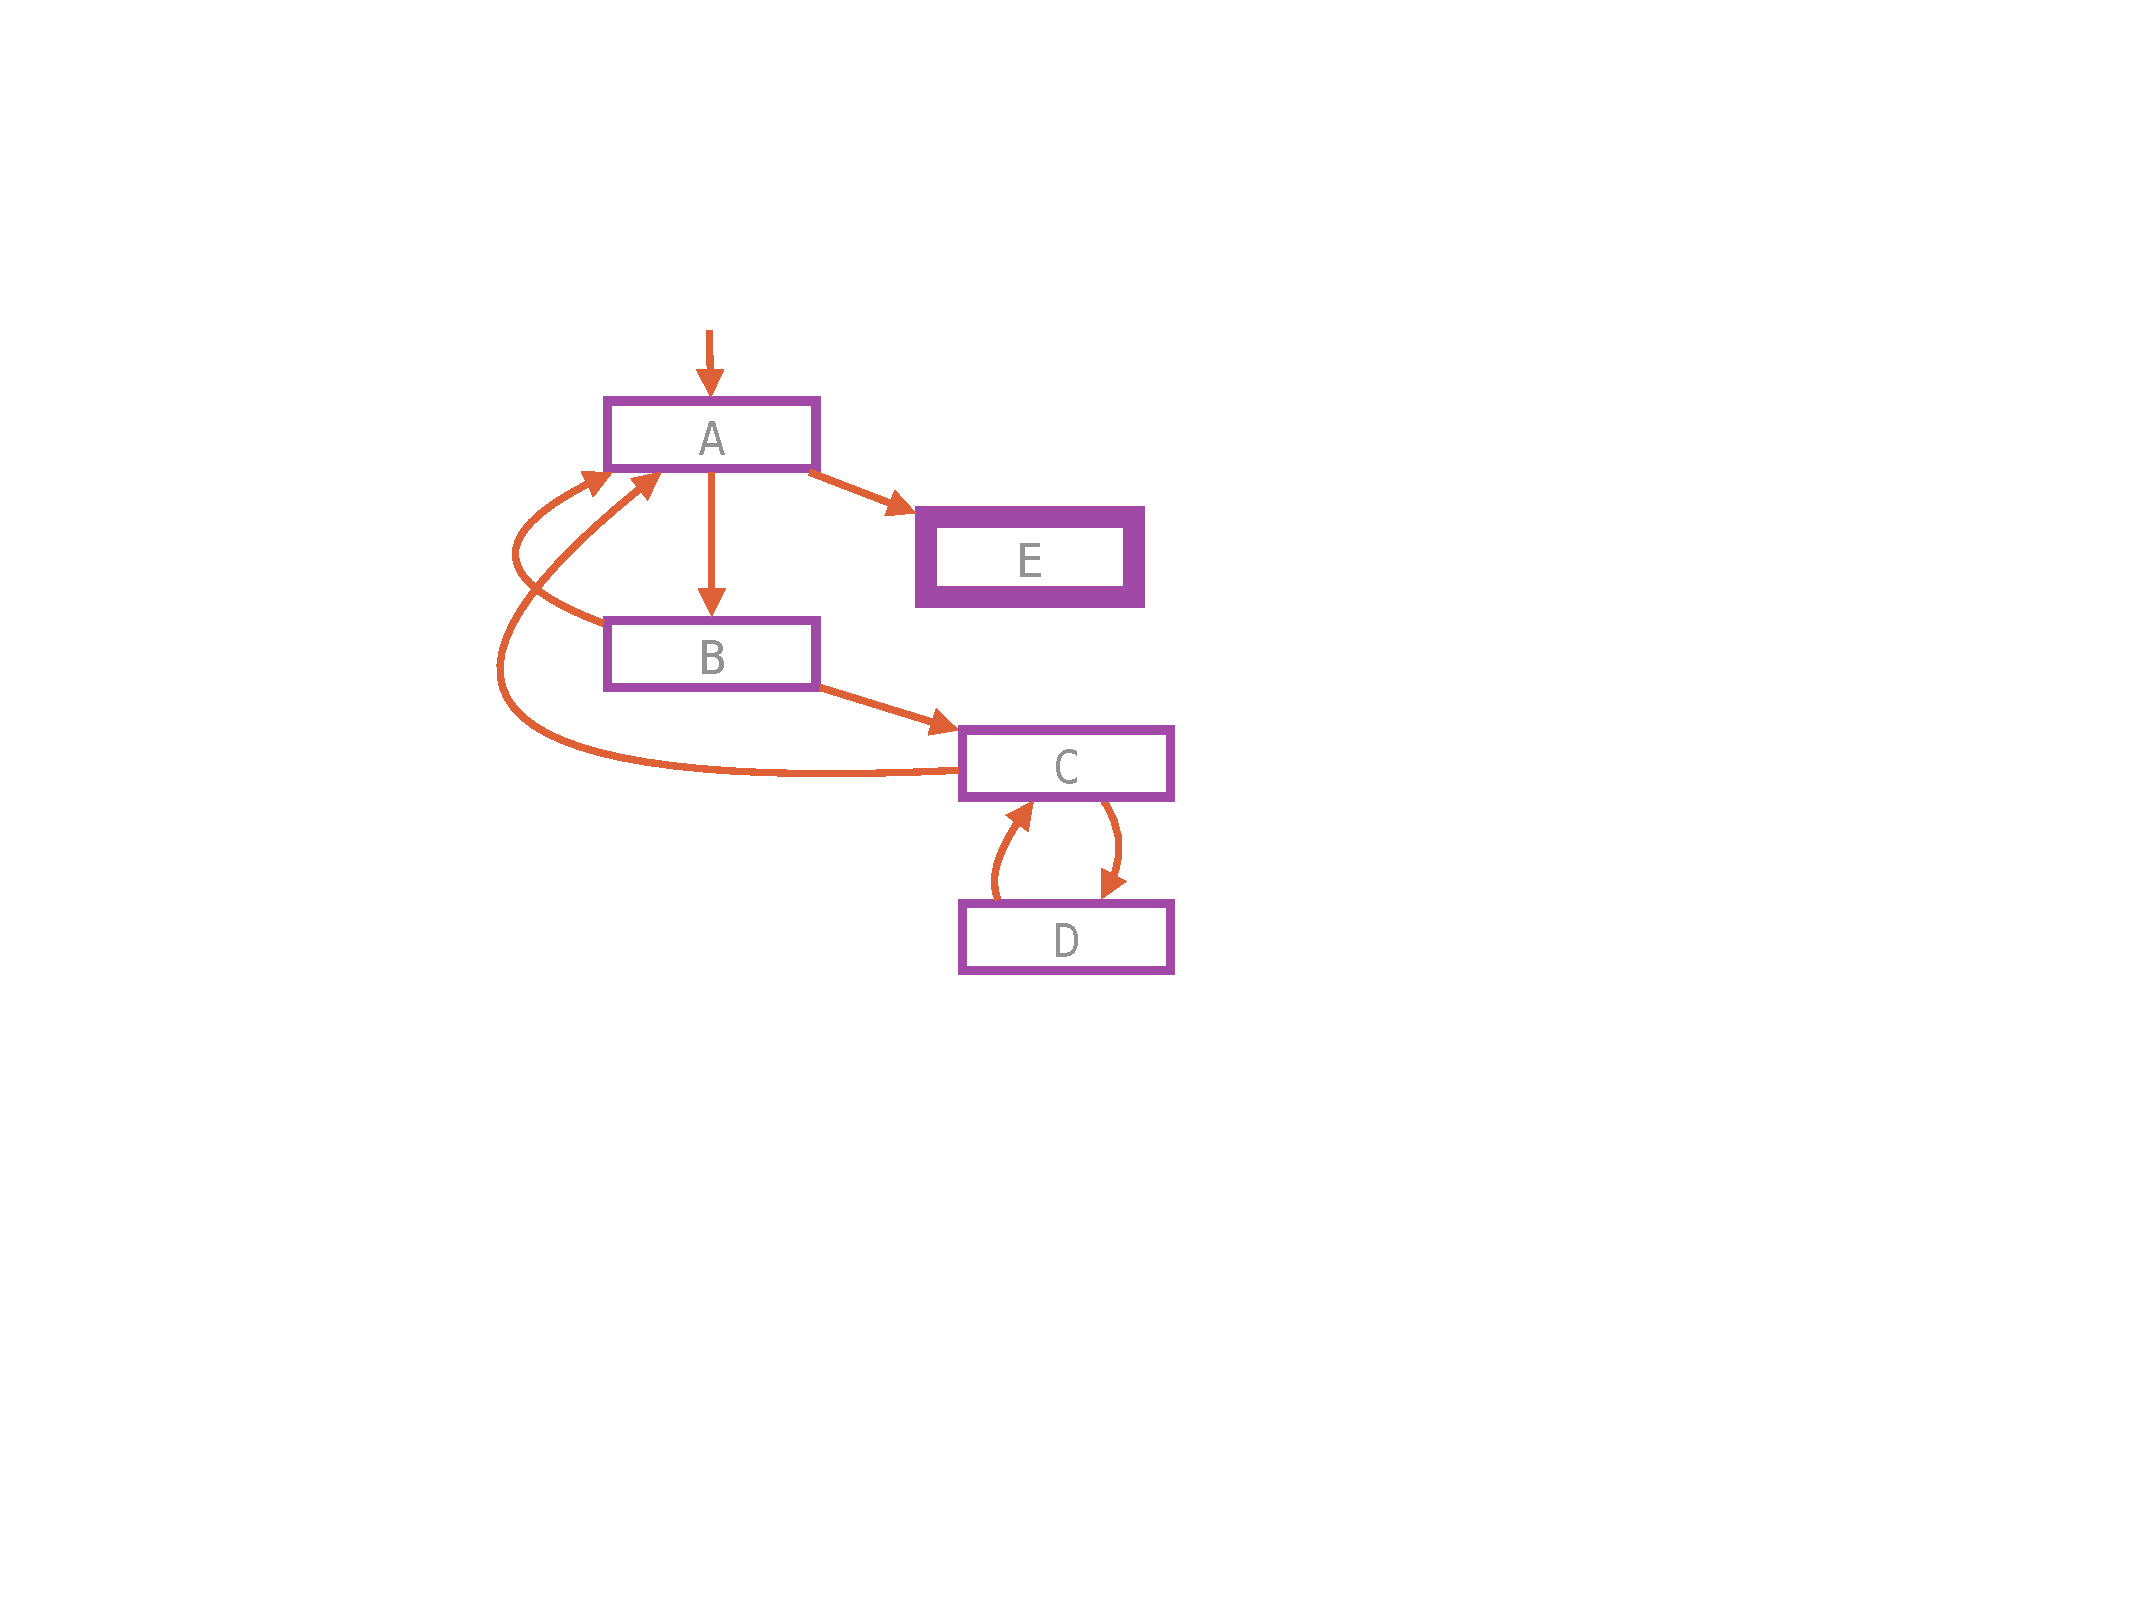
\includegraphics[width=7cm]{figures/sample-midterm-cfg-2.pdf}
  \end{figure}
\end{center}

\begin{parts}
\part[3] List all the simple paths in the CFG given above. %
  \answerspace{7} %
  \begin{solution} %
    \begin{itemize}
      \item[1] [A], [B], [C], [D], [E]  %
      \item[2] [A, E], [A, B], [B, A], [B, C], [C, A], [C, D], [D, C], %
      \item[3] [A, B, A], [A, B, C], [B, A, B] [B, A, E], [B, C, D],
        [B, C, A], [C, A, B], [C, A, E], [C, D, C], [D, C, A], [D, C,
        D] %
      \item[4] [A, B, C, D], [A, B, C, A], [B, C, A, B], [B, C, A, E], [C, A, B, C], [D, C, A, E],
        [D, C, A, B] % \\
      \end{itemize}
  \end{solution}

\part[3] List three test paths in the CFG given above. %
  \answerspace{7} %
  \begin{solution} %
    The test paths must start at node A and end at node E. Note that
    there is exactly one simple test path: [A, E]. Once you allow for
    the possibility of repeated nodes, however, the world is your
    oyster: [A, B, A, E], [A, B, C, D, C, A, E], etc.
    %
  \end{solution}

\part[3] List all the prime paths in the CFG given above. %
  \answerspace{7} %
  \begin{solution} %
    Recall that a prime path is a simple path that does not appear as
    a proper subpath of any other prime path.
    [A , B , A],
    [B, A, B],
    [B , A , E],
    [C , D , C],
    [D, C, D]
    [A , B , C , A],
    [A , B , C , D],
    [B , C , A , B],
    [B , C , A , E],
    [C, A, B, C],
    [D , C , A , B],
    [D , C , A , E]
  \end{solution}

  \newpage
\part[10] Write an example of a syntactically valid Java function
  that generates the control-flow graph above. If this is not
  possible, explain why. %
  \answerspace{23} %
  \begin{solution}
    Here is one possible solution:
    \begin{minted}{Java}
static int sillyAndAlsoFun(int a) {
  while (a <= 52){    // A
    if (a < 53) { // B
      while (a < 53) { // C
        a += 1;         // D
      }
    }
  }
  return a;             // E
}
\end{minted}
  \end{solution}

  \part[3] Provide test inputs that would generate the test paths
    you identified in 6a (or state they are infeasible).
    \answerspace{15}
    \begin{solution}
      \begin{itemize}
      \item [] \textbf{[A, E]}: (\mintinline{Java}{a}$\mapsto$
        \mintinline{Java}{53}, \mintinline{Java}{b}$\mapsto$ \mintinline{Java}{0}
      \item [] \textbf{[A, B, A, E]}: infeasible path
      \item [] \textbf{[A, B, C, D, C, A, E]}: \mintinline{Java}{a}$\mapsto$ \mintinline{Java}{52}
      \end{itemize}
    \end{solution}
  \end{parts}

\newpage
\question Consider the following control-flow graph annotated with
  def-use information. Unless otherwise noted, assume $def(l) =
  \emptyset$ and $use(l) = \emptyset$.
  \begin{figure}[ht]
    \begin{center}
      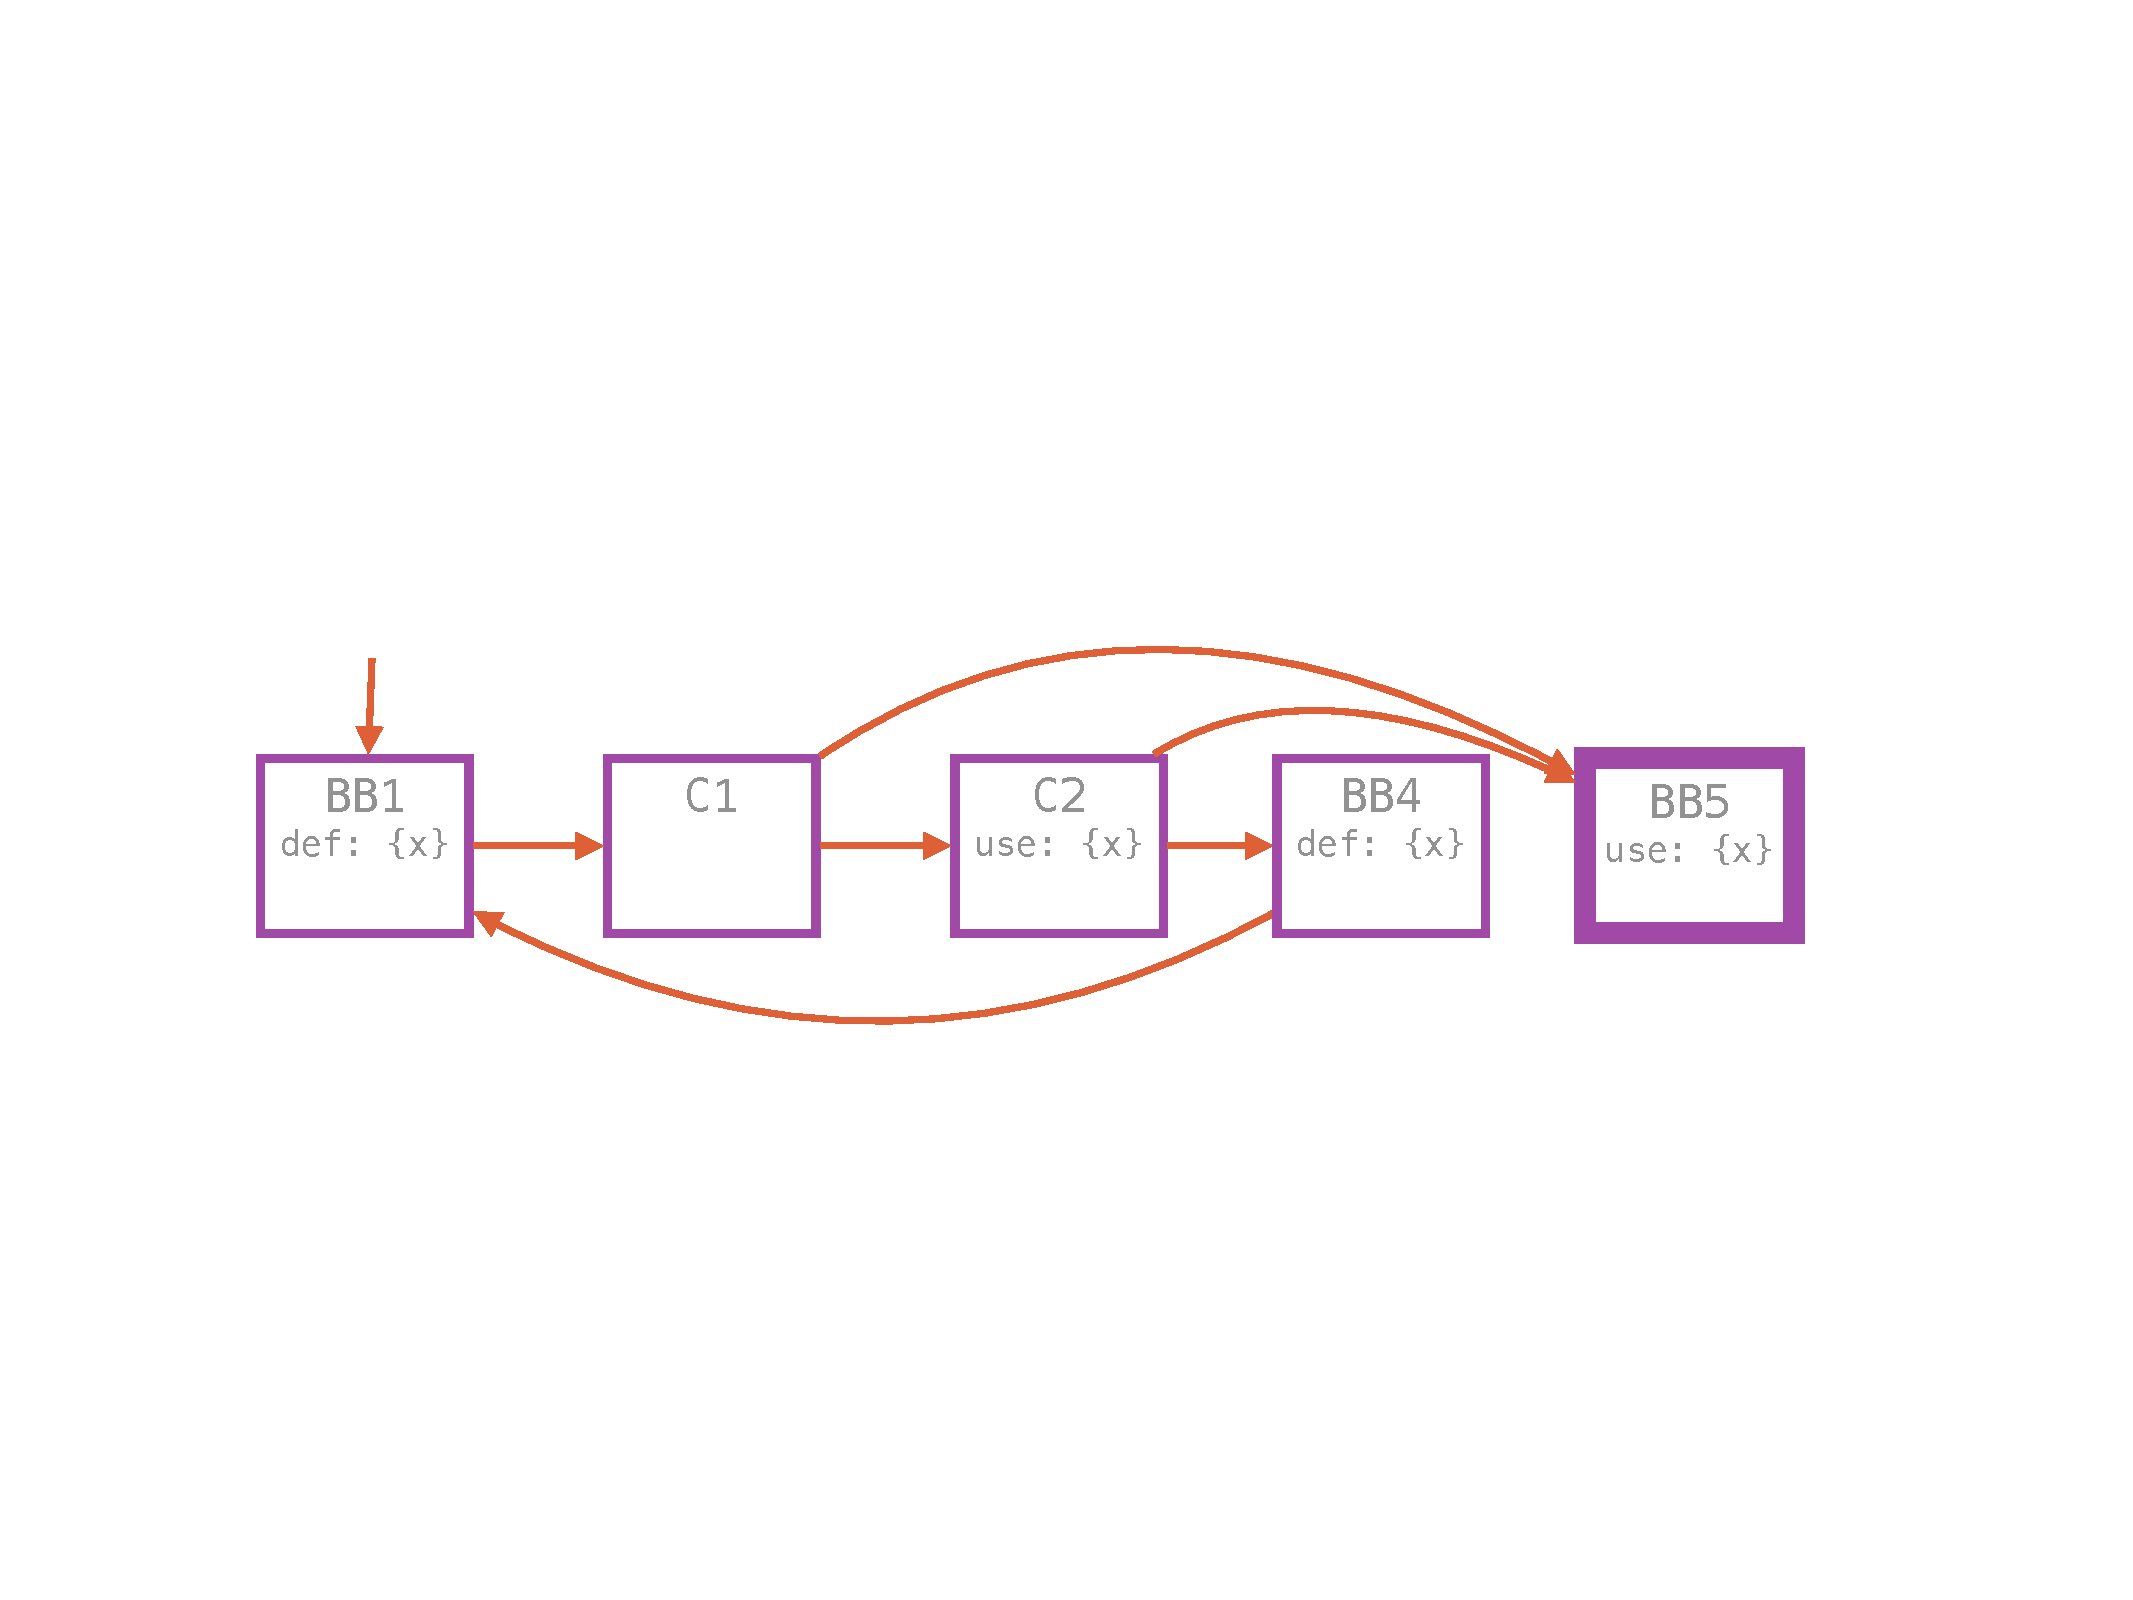
\includegraphics[width=.5\linewidth]{figures/sample-midterm-cfg}
    \end{center}
\end{figure}


\begin{parts}
    \part[3] List the test requirement set of all-defs coverage with respect to \mintinline{Java}{x}.
    \answerspace{12}
    \begin{solution}
      The test set includes a test case corresponding to one of the
      following paths: [0, 1, 2] or [0, 1, 5].
    \end{solution}

    \part[3] List the test requirement set of all-uses coverage with respect to \mintinline{Java}{x}.
    \answerspace{12}
    \begin{solution}
      The test set includes a test case corresponding to each of the
      following paths: [0, 1, 2] and either [0, 1, 5] or [0, 1, 2, 5].
      % Accept answer with just:
      % - TR = {[0, 1, 2], [0, 1, 4]}    OR
      % - TR = {[0, 1, 2], [0, 1, 2, 4]}
    \end{solution}

    \part[4] List the test requirement set of all-du-paths coverage with respect to \mintinline{Java}{x}.
    \answerspace{12}
    \begin{solution}
      The test set includes a test case corresponding to each of the
      following paths: [0, 1, 2],[0, 1, 5], and [0, 1, 2, 5].
\end{solution}
\end{parts}

\question[4] A tester defined three characteristics for the input
  parameter car: \textbf{Where Made}, \textbf{Energy Source}, and
  \textbf{Size}. The following partitioning for these characteristics
  has (at least) two mistakes. How would you correct them?

  \begin{center}
  \begin{tabular}{|c|c|c|}
    \hline
    \multicolumn{3}{|c|}{\textbf{Where Made}} \\\hline
    North America & Europe & Asia \\\hline
    \multicolumn{3}{|c|}{\textbf{Energy Source}} \\\hline
    gas & electric & hybrid \\\hline
    \multicolumn{3}{|c|}{\textbf{Size}}\\\hline
    2-door & 4-door & hatch back\\\hline
  \end{tabular}
\end{center}
\answerspace{15}
\begin{solution}
  Some potential mistakes:
  \begin{itemize}
  \item The ``Size'' describes the number of doors, as opposed to
    'compact', 'full-size', etc. and is thus arguably incomplete. More
    importantly, the ``Size'' categories are not mutually exclusive:
    it is possible to have a hatchback car with 4-doors, for
    example. The solution is to divy this up into proper, distinct
    size categories: [compact | mid-size | full-size | SUV/truck]
  \item The ``Where Made'' category is similarly incomplete: Brazil is
    a major car manufacturer, and Australia has been known to produce
    cars. One solution is to add additional categories, e.g.,
    [North America | Asia | Europe | South America | Other]
  \end{itemize}
\end{solution}

\newpage

\question[5] Explain how the coverage-guided fuzzers discussed in class work.
\answerspace{20}
\begin{solution} Grey-box fuzzers randomly test a program by
  iteratively generate new tests by mutating a corpus of test inputs
  derived from an initial set of test. They insert lightweight
  instrumentation to gather coverage feedback from each test execution
  to identify if a new test has covered a new node or branch, and use
  this information to update the corpus of test inputs and when
  generating the next test input.
  \end{solution}

  \newpage

\question[4]
  Provide a simple example of a program with a data race, where the
  lockset algorithm can help identify the problem. Provide and explain
  the results of the lockset algorithm on this program. %
  \answerspace{20} %
  \begin{solution}
    \begin{minted}{Java}
int balance = 0;
Lock lockA = new Lock();
Lock lockB = new Lock();

// Thread 1
void deposit() {
    lockA.lock();
    balance = balance + 100;
    lockA.unlock();
}

// Thread 2
void withdraw() {
    lockB.lock();
    balance = balance - 50;
    lockB.unlock();
  }
\end{minted}
    Suppose the test executes the first thread to completion, and then
    the second thread. The initial lockset for \mintinline{Java}{balance} will be \{A, B\},
    after executing the first thread, it will be \{A\}, and after
    executing the second, it will be \{ \}.


\end{solution}

\question[4] Provide a simple example of a program without a
  problematic data race, where the lockset algorithm will nevertheless
  flag a potential data race for the user. Provide and explain the
  results of the lockset algorithm on this program, and argue why this
  is a false positive.

  \answerspace{20}%
  \begin{solution}
    \begin{minted}{Java}
int balance = 0;
Lock lockA = new Lock();

// Thread 1 - This thread is always run before the other two
void init() {
    balance = 100;
}

// Thread 2
void deposit() {
    lockA.lock();
    balance = balance + 50;
    lockA.unlock();
}

// Thread 3
void withdraw() {
    lockA.lock();
    balance = balance - 25;
    lockA.unlock();
}
\end{minted}

    Here, the lockset algorithm will identify the first write to
    \mintinline{Java}{balance} as not being protected by any locks,
    and thus report a potential data race after \emph{every} test
    execution. This is okay however -- this use of
    \mintinline{Java}{balance} is actually protected by the control
    flow structure of the client program, which ensures that there can
    never be any concurrent accesses of  the variable while the first
    thread is running.
  \end{solution}




% \newpage
% \question[5] Describe two approaches to determine what are the properties of good bug reports. Explain how you would implement each.
% \answerspace{16}
% \begin{solution}Examples: (a) conducting developer surveys and (b) studying the properties of bug reports in bug repositories.}


\newpage



\if 0 %%%%%%%%%%%%%%%%%%%%%%%%%%%%%%%%%%%%%%%%%
	\question[10]
	\answerspace{30}
	\begin{solution}}

	\question
	\begin{parts}
		\part[6]
		\answerspace{20}
		\begin{solution}}

		\part[2]
		\answerspace{10}
		\begin{solution}
                \end{answer}

	\end{parts}
\fi %%%%%%%%%%%%%%%%%%%%%%%%%%%%%%%%%%%%%%%%%

	\newpage
	\begin{center}
		[EMPTY PAGE 1]
	\end{center}

	\newpage
	\begin{center}
		[EMPTY PAGE 2]
	\end{center}

\end{questions}





\end{document}
